\documentclass[titlepage,a4paper,12pt,thmsb]{report}

\usepackage{graphicx}
\usepackage{graphics}
\usepackage[english]{babel}
\usepackage{float,epsfig, floatflt,here}
\usepackage{amsmath}
\usepackage{a4}
\usepackage{fancyhdr}
\usepackage{makeidx}
\usepackage{hyperref}
\usepackage{moreverb}
%\usepackage{loremipsum}
\usepackage{tabularx}
\usepackage{tabulary}
\usepackage{algorithm}
\usepackage{algorithmic}

\textwidth 16cm \textheight 22.5cm \selectlanguage{english}
\topmargin 0cm \headheight 0.5 cm \oddsidemargin 0cm
\evensidemargin 0cm
\renewcommand{\baselinestretch} {1.2} \setlength{\parindent}{0.0cm}
\setlength{\parskip} {0.5 cm}
%\renewcommand{\thesection}{\arabic{section}}
\renewcommand{\thechapter}{\arabic{chapter}}
\setcounter {secnumdepth}{5} \setcounter{tocdepth}{5}
\let\oldTitle\title
\renewcommand{\title}[1]{\newcommand{\myTitle}{#1}\oldTitle{#1}}
\newcommand{\leftscripts}[3]{{\vphantom{#3}}^{#1}_{#2}{#3}}

%%% Fancy Header %%%%%%%%%%%%%%%%%%%%%%%%%%%%%%%%%%%%%%%%%%%%%%%%%%%%%%%%%%%%%%%%%%
% Fancy Header Style Options
\pagestyle{fancyplain}                  % Sets fancy header and footer
%\fancyfoot{}                           % Delete current footer settings
\renewcommand{\chaptermark}[1]{         % Lower Case Chapter marker style
  \markboth{\chaptername\ \thechapter.\ #1}{}} %
\renewcommand{\sectionmark}[1]{         % Lower case Section marker style
  \markright{\thesection.\ #1}}         %
\fancyhead[LE,RO]{\thepage}             % Page number (boldface) in left on even
                                        % pages and right on odd pages
%\fancyhead[RE]{\bfseries\leftmark}     % Chapter in the right on even pages
\fancyhead[RE]{\leftmark}               % Chapter in the right on even pages
%\fancyhead[LO]{\bfseries\rightmark}    % Section in the left on odd pages
\fancyhead[LO]{\rightmark}              % Section in the left on odd pages

\renewcommand{\headrulewidth}{0.1pt}    % Width of head rule
\renewcommand\footrulewidth{0.1pt}
%\fancyfoot[CE,CO]{\myTitle}{}
\fancyfoot[CE,CO]{Network Science}{}
\makeindex
%%%%%%%%%%%%%%%%%%%%%%%%%%%%%%%%%%%%%%%%%%%%%%%%%%%%%%%%%%%%%%%%%%%%%%%%%%%%%%%%%%%%%%%
%\let\oldAuthor\author
%\renewcommand{\author}[1]{\newcommand{\myAuthor}{#1}\oldAuthor{#1}}
%%%%%%%%%%%%%%%%%%%%%%%%%%%%%%%%%%%%%%%%%%%%%%%%%%%%%%%%%%%%%%%%%%%%%%%%%%%%%%%%%%%%%%%
\begin{document}
\pagenumbering{roman}
\begin{titlepage}
\thispagestyle{empty}
%\vspace*{0.7cm}
\begin{center}
%{\centering
%\large
{\LARGE \bf{Report of Network Science Assignment}} \\
\vspace{1.5cm}
%\it{A project report submitted in partial fulfillment \\ for the requirements for the degree of \\ Master of IT in Business} \\
%\large \bf{ Report of } \\
%\large \bf{CS212\\ Intelligent Data Analysis} \\
%\vspace{0.3cm}
%\sc
\large \sc{made by} \\
\vspace{0.3cm}
\rm
{\large \bf {Ziyuan Ye}}\\
%{\large \bf {01010410}}
\vspace{0.3cm}
%\sc
\bf{11610203@mail.sustc.edu.cn} \\

\vspace{1cm}

{\large\sc{under the guidance of}} \\
\vspace{.5cm}

\hspace{.05cm} {\bf {Shan He}}\\
\hspace{.05cm} {\sc and}\\
\hspace{.05cm} {\bf {Chengbin Hou}}\\
%\vspace{0.5cm}
%\vspace{0.5cm}
%\universityseal\ \\

\begin{figure}[h]
%\hspace{6cm}
%\vspace{5cm}
{\centering {\includegraphics[width=0.5\linewidth,angle=0]{logo/logo.png}}\par}
\end{figure}
%\vskip 0.5cm
%\large{\bf Department of Mathematics \& Computing} \\
\large{\bf Department of Computer Science and Engineering} \\
\vskip 0.5cm
%\Large{\bf Indian Institute of Technology Guwahati}\\
\Large{\bf Southern University of Science and Technology}\\
%\vskip 0.5cm
{\centering \sc{Shenzhen, China, July 2018}}
%} %%% this is end of centering environment
\end{center}
\pagebreak
\end{titlepage}


\chapter*{Abstract}
\addcontentsline{toc}{chapter}{\numberline{}CERTIFICATE}
This assignment focus on analsying the data set with the technique such as {\bf Page Rank}, {\bf Find Eigenvector Centrality} and {\bf Find In and Out degree}. I try to combine the above methods to work out the top 10 rank of a data set which is called {\bf Top Four Cities}.))
This data set seems very confusing initially. However, by using the above techniques, we gradually can find the top 10 nodes which has the highest rank in all the data set.


%\chapter*{Detail of Red Wine Quality Data Set}
%{\large \bf {12 Dimensions}}
%\begin{itemize}
%\item{Fixed acidity (g(tartaric acid)/dm3), range from 4.6 to 15.9 mean value is	8.3}
%\item{Volatile acidity (g(acetic acid)/dm3),  range from	0.1 to 1.6 mean value is 0.5}


%\end{itemize}
{\large \bf {Data Set Source:}}
\newline{}
{\hspace*{0.7cm}{\url{/Dataset/topfourcites.txt}} }
\newline{}
\vspace{0.5cm}


%\addcontentsline{toc}{chapter}{\numberline{}Abstract}

%\addcontentsline{toc}{chapter}{\numberline{}Executive Summary}

%\chapter*{Preface}
%\addcontentsline{toc}{chapter}{\numberline{}Preface}
%{\bf ``Problems worthy of attack prove their worth by hitting back"}


%%-------------------------- Table of contents ---------------------------------%%
%\newpage
%%
%\centerline{{\bf {\large CONTENTS}}}
%%
%\tableofcontents{}
%\newpage
%\addcontentsline{toc}{chapter}{\numberline{}Table of Contents}
%\tableofcontents
%\makeindex
\newpage

\pagenumbering{arabic}
%\chapter*{Preprocessing Data}
%\section*{Normalization}
%The {\bf unit} and {\bf scale} of the data is different, this method can make different characters have the same scale.  Only in this way, %the comparison can be valid.
%$$
 % \widehat{E[X_i]} \approx \frac{1}{N} \sum_{j=1}^{N} X_i^j \\
 % \widehat{Var[X_i]}   \approx \frac{1}{N} \sum_{j=1}^N (X_i^j - \widehat{E[X_i]})^2 = \sigma^2 \\
 % \widehat{X_{i,nor}^j}  \approx \frac{X_i^j - E[X_i]}{\sigma}
%$$
%It's important to shift every attributes of the data to be centered:
%$$\mathop{\mathbb{E}[X_i] = 0, i = 1,2,...d.}$$It's also important to scale the density of every attributes of the data so the standard %deviation (or variance) need to be rescaled: $$\mathop{\mathbb{Var}[X_i] = 1, i = 1,2,...d.}$$Now every attribute is standardized to $%\mathop{\frac{X_i - \mu}{\sigma}}$.
\chapter{ Introduce the PageRank Algorithm }
\section{ Flowchart }

\begin{center}
\begin{figure}[h]
{\centering {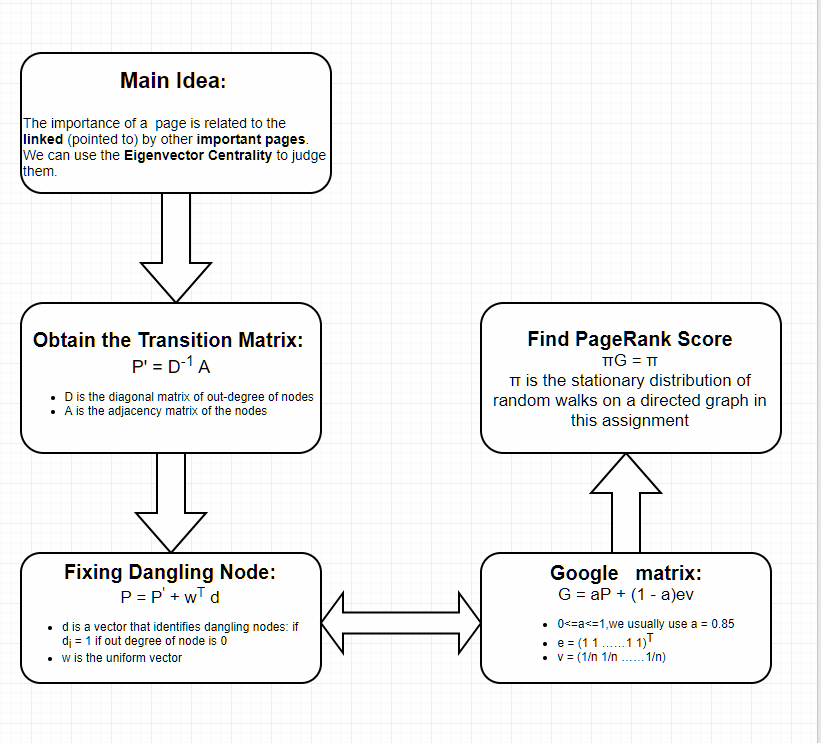
\includegraphics[width=0.65\linewidth,angle=0]{logo/stream_graph.png}}\par}
\end{figure}
{\centering{\bf{Figure: Flowchart}}}
\end{center}

The flowchart cover each page rank step. It also cover the parameters and how I use select them.

\newpage
\section{ Pseudo-code }

\begin{algorithm}
\caption{Calculate  $pagerank$} 
\label{alg1}
\begin{algorithmic}
\REQUIRE $v = (1/n, 1/n  .... 1/n),
			e = (1,1,1,1.....1 1),
			W = (1/n, 1/n  .... 1/n)$ 
\STATE $d[i]$ $is$ $the$ $out$ $degree$ $of$ $node$ $i$
\STATE $y \Leftarrow 1$ 
\IF{$out$ $degree$ $of$ $node$ = $0$} 
\STATE $d[i] \Leftarrow 1$ 
\ELSE 
\STATE $d[i] \Leftarrow 0$ 
\ENDIF 
\STATE	$D'$  $is$ $the$ $diagonal$ $matrix$ $of$ $out-degree$ $of$ $nodes$
\STATE  $P' \Leftarrow D' \times A$ 
\STATE  $P \Leftarrow P' + W^T  \times d$ 
\STATE  $G \Leftarrow \alpha \times P + 1-\alpha  \times ev$ 
\STATE  $\pi(0) = (1/n, 1/n  .... 1/n)$ 
\WHILE{$True$} 
\STATE $p(i+1)\Leftarrow p(i) \times G$ 
\IF{$abs(\pi(i+1) - \pi(i)) < error$} 
\STATE $break$ 
\ENDIF 
\ENDWHILE
\RETURN $\pi$
\end{algorithmic}
\end{algorithm}

\newpage

\chapter{Visualization}

In this chapter, I visualize a tables combine with a graphs of the top ten node in each algorithm
\newpage


\begin{center}
{\centering{\begin{tabular}{ |l|l| }
  \hline
  \multicolumn{2}{|c|}{Top ten in degree of node} \\
  \hline
  \hline
  \multicolumn{1}{|c|}{Node} &
  \multicolumn{1}{|c|}{value} \\
  \hline
Meyer DS 2004 & 8.03124821796318\\
Earl J 2004 &  6.382854503328885\\
Kalev A 2006 & 5.146559217353166\\
Cress DM 2000 & 3.498165502718872\\
Sampson RJ 2005 & 3.498165502718872\\
Charles CZ 2003 & 3.0860670740602987\\
King BG 2007 & 3.0860670740602987\\
Mcadam D 2001 & 2.880017859731012\\
Benford RD 2000 &  2.6739686454017257\\
Logan JR 2004 & 2.467919431072439\\
  \hline
\end{tabular}}}
\end{center}
\begin{center}
{\centering{\bf{Table: Top ten in degree of node}}}
\end{center}

\begin{center}
\begin{figure}[h]
{\centering {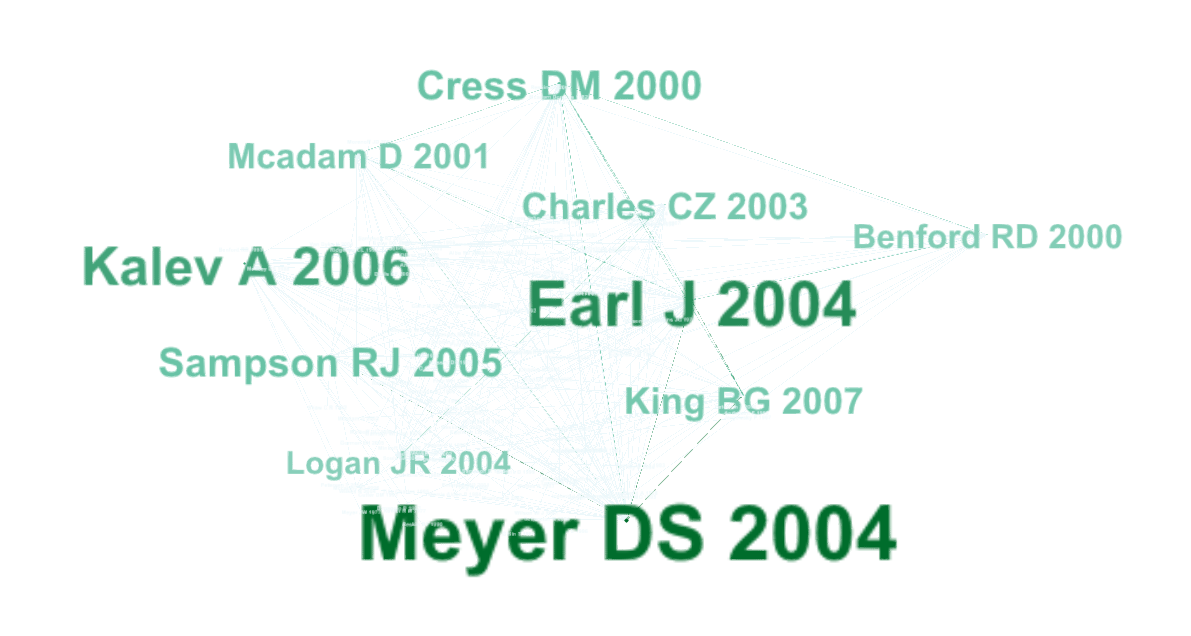
\includegraphics[width=0.6\linewidth,angle=0]{logo/in.png}}\par}
\end{figure}
\end{center}
\begin{center}
{\centering{\bf{Figure In degree of top ten node}}}
\end{center}

\newpage


\begin{center}
{\centering{\begin{tabular}{ |l|l| }
  \hline
  \multicolumn{2}{|c|}{Top ten out degree of node} \\
  \hline
  \hline
  \multicolumn{1}{|c|}{Node} &
  \multicolumn{1}{|c|}{value} \\
  \hline
Mccarthy JD 1977 & 8.012879874411901\\
Mcadam Douglas 1982 & 6.008786197075345\\
Tilly C 1978 & 5.700464092869721\\
Wilson W J 1987 & 5.083819884458474\\
Denton Nancy A 1993 & 4.7754977802528495\\
Dimaggio PJ 1983 & 4.158853571841602\\
Meyer JW 1977 & 4.00469251973879\\
Granovetms 1973 & 3.850531467635978\\
Mccarthy JD 1996 & 3.2338872592247303\\
Gamson W 1990 & 3.0797262071219182\\
  \hline
\end{tabular}}}
\end{center}
\begin{center}
{\centering{\bf{Table: Top ten out degree of node}}}
\end{center}

\begin{center}
\begin{figure}[h]
{\centering {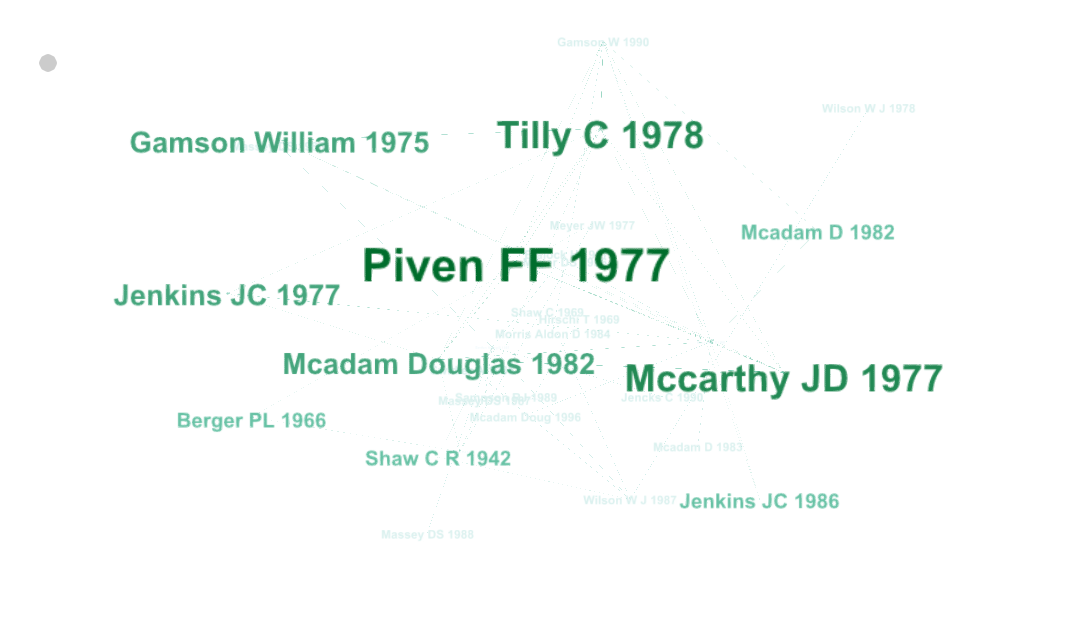
\includegraphics[width=0.6\linewidth,angle=0]{logo/out.png}}\par}
\end{figure}
{\centering{\bf{Figure Out degree of top ten node}}}
\end{center}

\newpage


\begin{center}
{\centering{\begin{tabular}{ |l|l| }
  \hline
  \multicolumn{2}{|c|}{Top ten Eigenvector centrality of node} \\
  \hline
   \hline
  \multicolumn{1}{|c|}{Node} &
  \multicolumn{1}{|c|}{value} \\
  \hline
Meyer DS 2004 & 0.2714494\\
Mccarthy JD 1977 & 0.27114936\\
Cress DM 2000 & 0.24436234\\
Earl J 2004 & 0.23883461\\
Tilly C 1978 & 0.23256826\\
Mccarthy JD 1996 & 0.222541\\
Mcadam Douglas 1982 & 0.2130869\\
Gamson W 1990 & 0.20264384\\
Tarrow S 1998 & 0.1793854\\
Mcadam D 2001 & 0.15747336\\
  \hline
\end{tabular}}}
\end{center}
\begin{center}
{\centering{\bf{Table: Top ten Eigenvector centrality of node}}}
\end{center}
\begin{center}
\begin{figure}[h]
{\centering {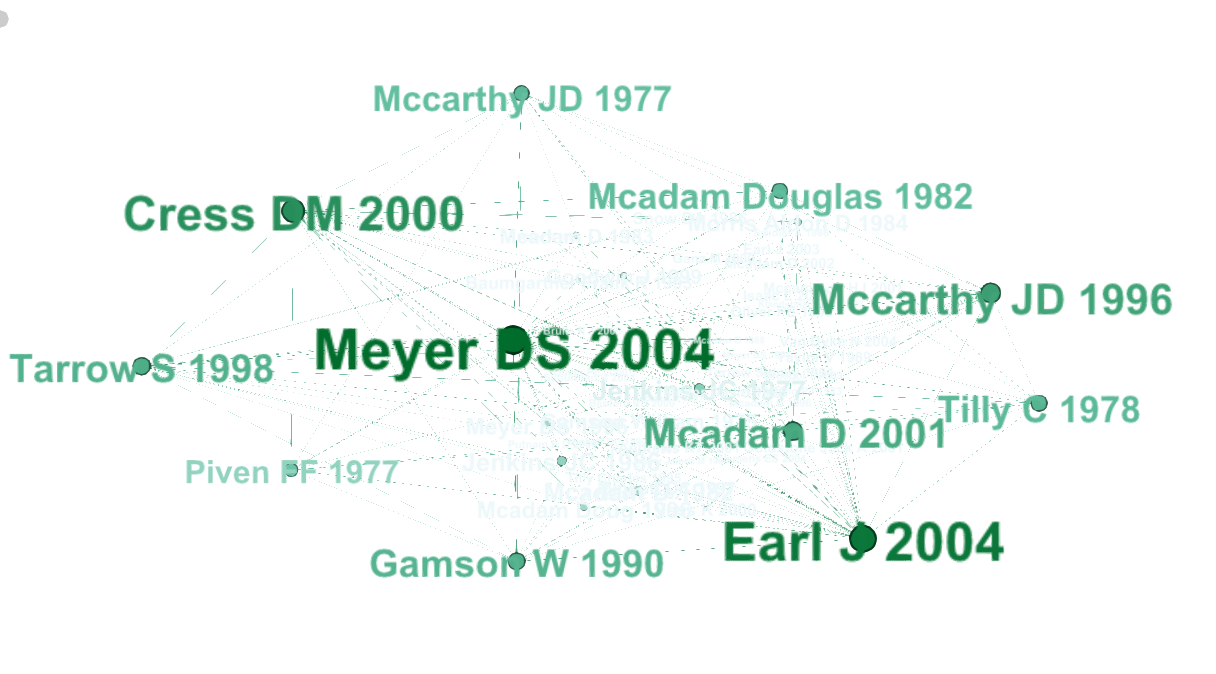
\includegraphics[width=0.6\linewidth,angle=0]{logo/centrality.png}}\par}
\end{figure}
{\centering{\bf{Figure Eigenvector centrality of top ten node}}}
\end{center}

I try the iteration equals 100 and 200 and find the same result, which means that in at most 100 iterations the eigenvector centrality will come to converge.
\newpage

\begin{center}
{\centering{\begin{tabular}{ |l|l| }
  \hline
  \multicolumn{2}{|c|}{Top ten Page Rank of node} \\
  \hline
   \hline
  \multicolumn{1}{|c|}{Node} &
  \multicolumn{1}{|c|}{value} \\
  \hline
Meyer DS 2004 & 0.78125451\\
Earl J 2004 & 0.31142786\\
Andrews KT 2004 & 0.17355846\\
King BG 2007 & 0.1697048\\
Mcadam D 2001 & 0.16243874\\
Cress DM 2000 & 0.15626345\\
Davis GF 2005 & 0.14311321\\
Mccammon HJ 2001 & 0.12880348\\
King BG 2005 & 0.11845306\\
Sampson RJ 2002 & 0.11700992\\
  \hline
\end{tabular}}}
\end{center}
\begin{center}
{\centering{\bf{Table: Top ten Page Rank of node}}}
\end{center}

\begin{center}
\begin{figure}[h]
{\centering {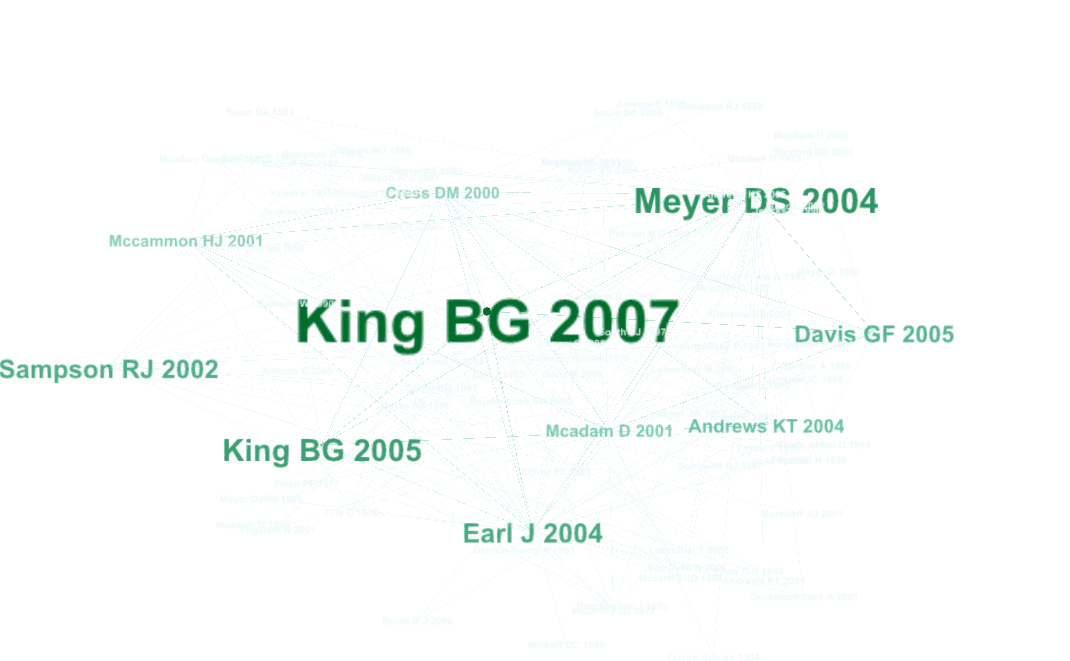
\includegraphics[width=0.6\linewidth,angle=0]{logo/page_rank.png}}\par}
\end{figure}
{\centering{\bf{Figure Page Rank of top ten node}}}
\end{center}

I try the iteration equals 100 and 200 and find the same result, which means that in at most 100 iterations the eigenvector centrality will come to converge.

\newpage


\chapter{Conclusion}
\section{ Abstract of In Degree, Out Degree and Eigenvector Centrality }

As we learn, in degree means how many a node be pointed by other nodes. Out degree means how many a node pointing to other nodes. Eigenvector centrality means the importance of a node depends on the importance of its neighbors.
\newpage
\section{Comparison of In Degree, Out Degree and Eigenvector Centrality }

As the table show above, we can find that top ten out degree node have numeral same nodes compare with eigenvector centrality.  Thus, we can make an assumption that the higher out degree of a node is, the higher eigenvector centrality it might be.  In the same way we can find that top ten out degree of nodes also similar with top ten eigenvector centrality.  However the in degree and out degree rank result has few same nodes.
\newline
\newline
Finally,we can make a conclusion that the importance of a node is judge by both in degree and out degree rather than just one of them.

\newpage


\chapter{Epilogue}
Due to the limitation of the time, my result may not the same as the result called by library.

However, I cover all the requirements!  Also, I try my best to approximate my result to the standard result.  Fortunately, I found my result is similar to the standard one.

If it is possible, I am looking forward to be your students in the future. 

Finally, I sincerely express my appreciation here to Chengbin and Shan He.
\vspace*{0.5cm}\\
{\large \bf {Code \& Related Files:}}
\newline{}
{\hspace*{0.7cm}{\url{https://github.com/Voldet/NS_project}} }

\bibliographystyle{plain}
\bibliography{cimne}
\end{document}
